\documentclass{article}

\usepackage[final]{neurips_2019}

\usepackage[utf8]{inputenc}
\usepackage[T1]{fontenc}
\usepackage{hyperref}
\usepackage{url}
\usepackage{booktabs}
\usepackage{amsfonts}
\usepackage{amsmath, bm, bbm}
\usepackage{amssymb}
\usepackage{nicefrac}
\usepackage{microtype}
\usepackage{graphicx}
\usepackage{xcolor}
\usepackage{lipsum}
\usepackage{makecell}

\newcommand{\note}[1]{\textcolor{blue}{{#1}}}

\title{
  Exploring CNNs in Question Answering \\
  \vspace{1em}
  \small{\normalfont Stanford CS224N Default Project}  % Select one and delete the other
}

\author{
  Joseph Pagadora, $\;$ Steve Gan \\
  Stanford University \\
  \texttt{jcp737@stanford.edu}$\;\;\;\;$
  \texttt{zgan@stanford.edu} \\
  % Examples of more authors
%   \And
%   Name \\
%   Department of Computer Science \\
%   Stanford University \\
%   \texttt{name@stanford.edu} \\
%   \And
%   Name \\
%   Department of Computer Science \\
%   Stanford University \\
%   \texttt{name@stanford.edu}
}

\begin{document}

\maketitle

% \begin{abstract}
%   Required for final report
% \end{abstract}

\section{Research paper summary}

\begin{table}[h]
    \centering
    \begin{tabular}{ll}
        \toprule
        \textbf{Title} & \makecell{QANet: Combining Local Convolution with Global Self-Attention for \\ Reading Comprehension} \\
        \midrule
        \textbf{Authors} & \makecell{Adams Wei Yu, David Dohan, Minh-Thang Luong, Rui Zhao, \\ Kai Chen, Mohammad Norouzi, Quoc V. Le} \\
        \textbf{Venue} & ICLR 2018 \\
        \textbf{Year}  & 2018 \\
        \textbf{URL}   & \url{https://arxiv.org/pdf/1804.09541.pdf} \\
        \bottomrule
    \end{tabular}
    \vspace{1em}
\end{table}

\paragraph{Background.}
This paper introduces a new architecture (QANet) to question-answering completely without the use of RNNs \cite{YU}. Many of the prior works toward this problems involve the use of RNNs and their ability to encode sequential data, but as a consequence, this results in longer training and inference time. At the time when RNNs with attention were the best way to learn from language data, this paper proposed to use convolutional layers with self-attention in question-answering models to achieve fast training and inference. The higher speed makes training on a larger dataset feasible, and so a data-augmentation method via back-translation is explored.

\begin{figure}[h]
\centering
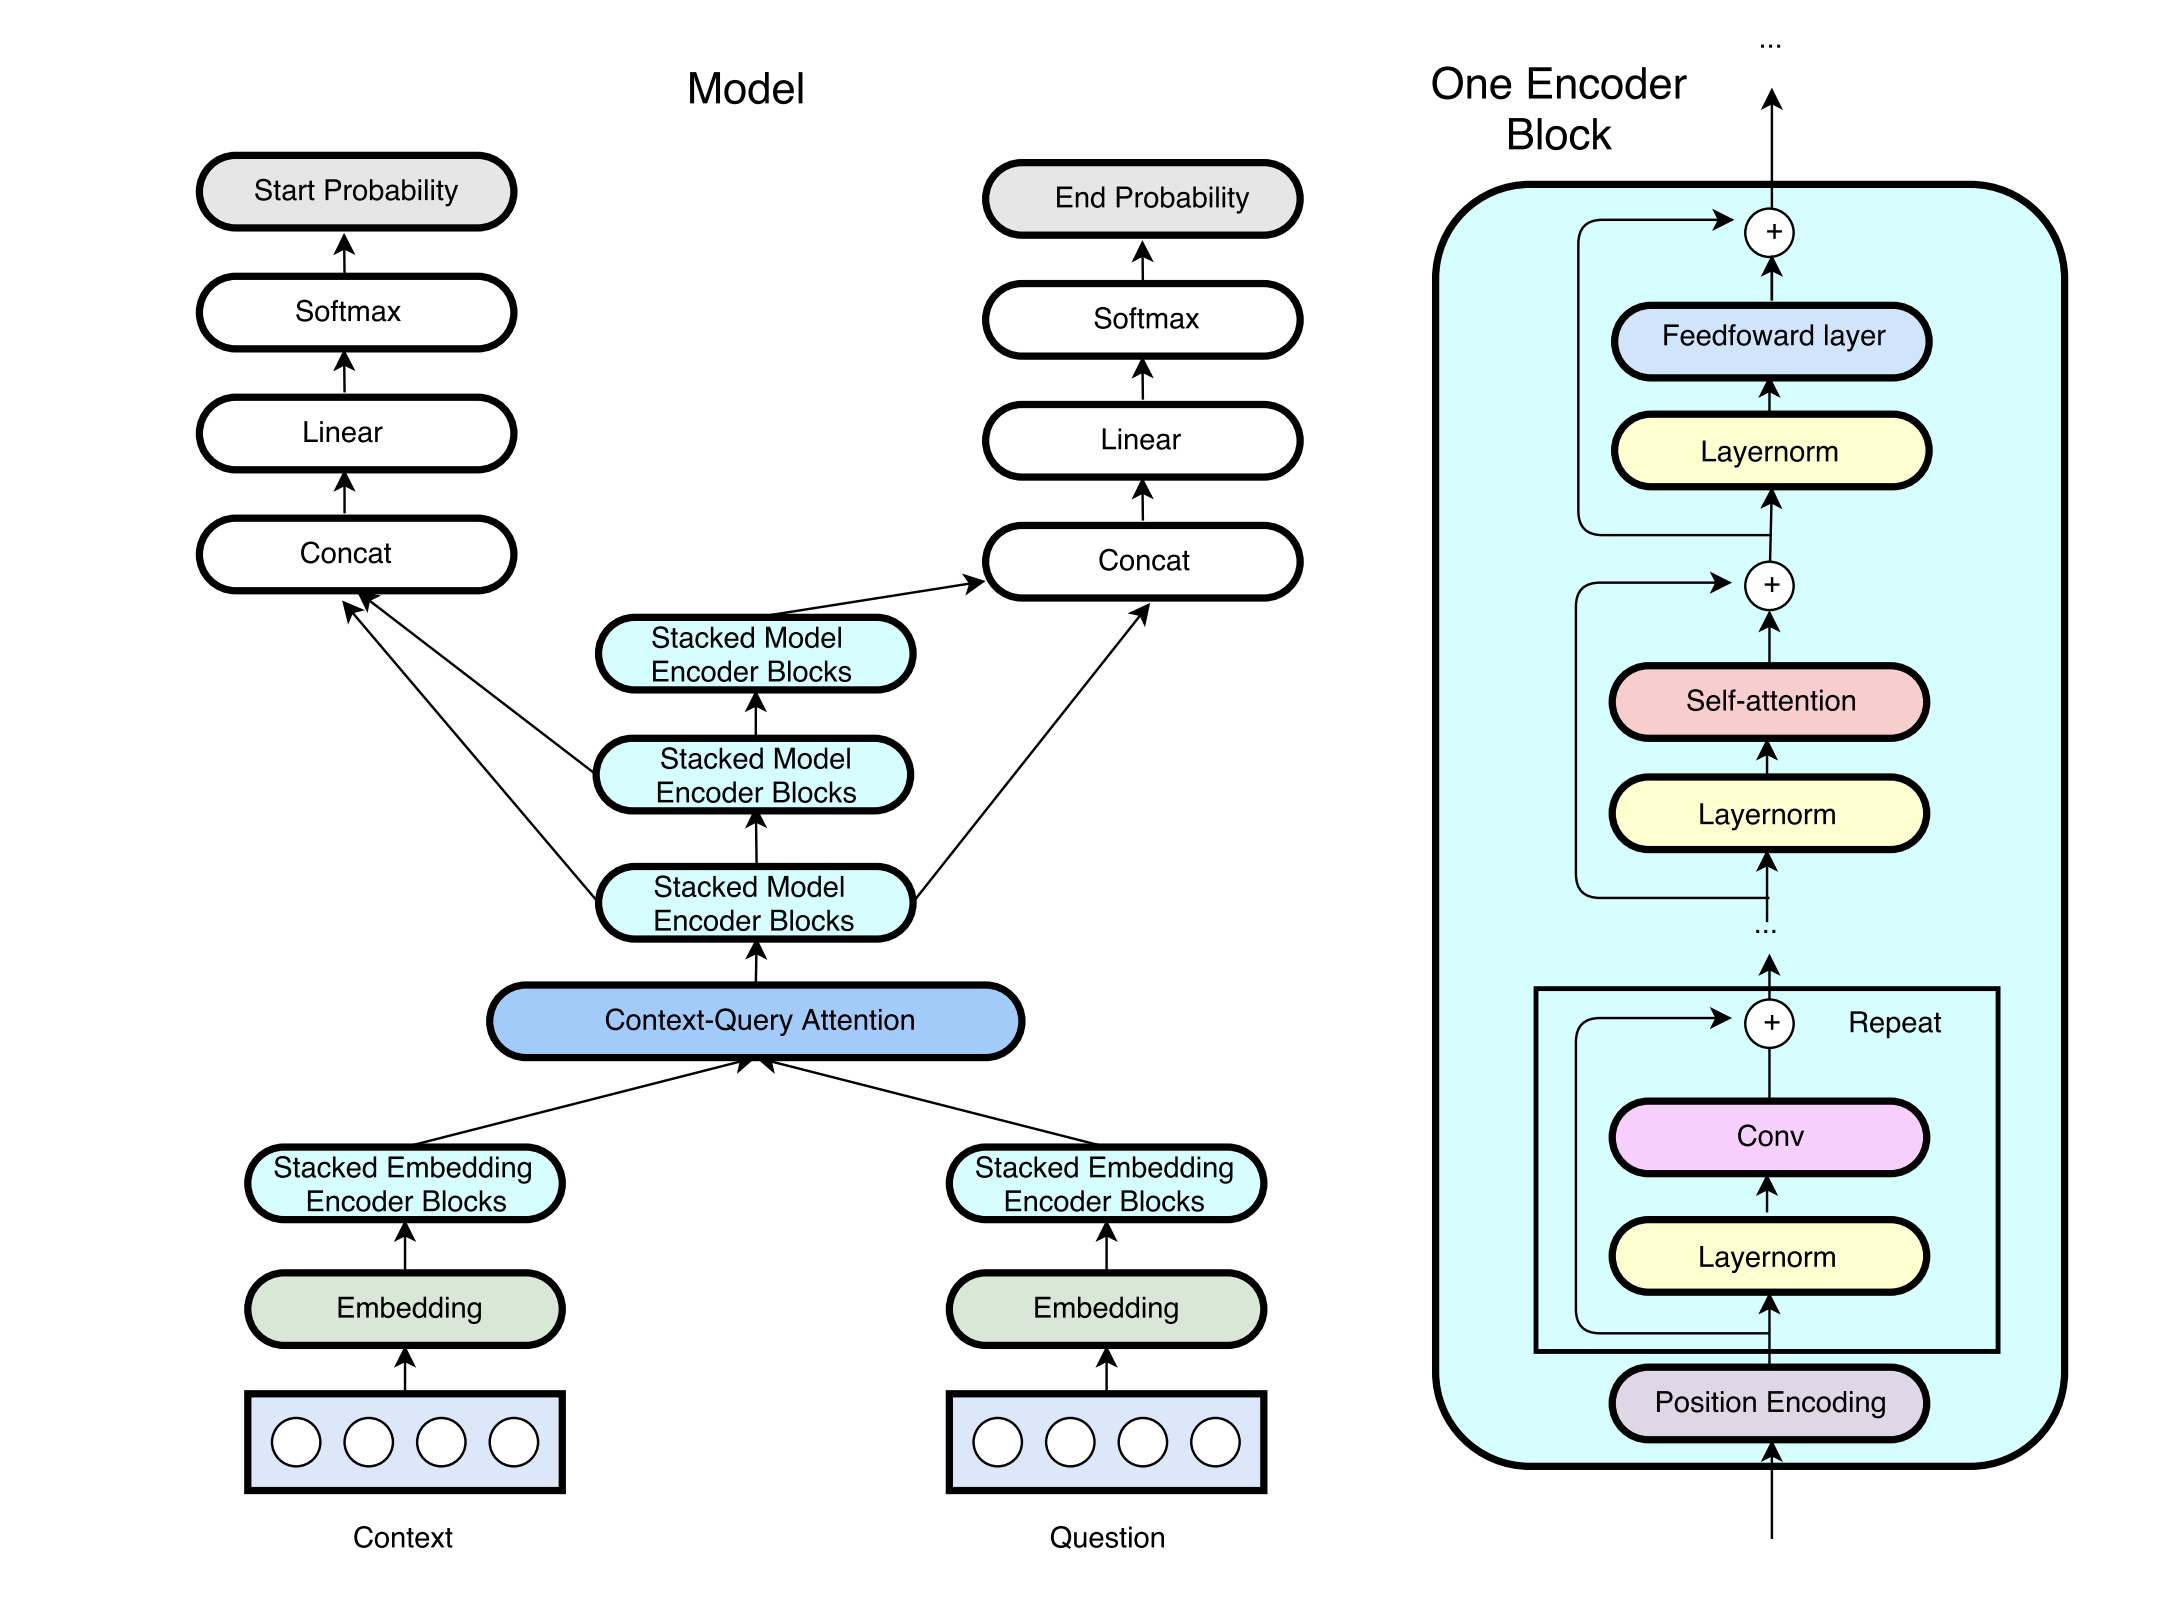
\includegraphics[scale=0.23]{model_diagram}
\caption{Left: Architecture of QANet with convolution and self-attention. Right: Encoder block that is used throughout the model.}
\end{figure}

\paragraph{Summary of Contributions.}
This paper proposes a new and faster way to approach the task of reading comprehension and question-answering without the use of a recurrent model. This approach is motivated by slow training and inference of RNNs. The paper outlines a new method that uses encoders consisting only of convolutional layers for local analysis of the input, along with self-attention for global analysis. This resulted in an increase in training speed about 3 to 13 times and in inference speed about 4 to 9 times compared to the standards set by previous high-accuracy methods that used RNNs.

Because of this drastic increase in efficiency, the model is able to be trained on a much larger dataset. Using the SQuAD dataset, the authors devised a data-augmentation approach: they translated the data to another language, and then translated it back to English, obtaining a paraphrase of the original data. Obviously, they hoped for an imperfect translator, that is, one that does not provide an invertible mapping. In other words, the synthesized datapoint has different phrasing than that of the original. This technique allows the model to acquire more data, thus improving performance on the question-answering task. The authors were able to achieve a 84.6 F1 score on the SQuAD test set after training on the augmented SQuAD training set.

Figure 1 shows a summarized diagram of the architecture of QANet. The raw input is given as $(C,Q)=$ (context, question) pairs, where the context $C=\{c_1,...,c_n\}$ consists of, say, $n$ words, and the model is to output a consecutive span $S=\{c_s,...,c_e\}\subseteq C$ containing the answer to the question $Q.$ The QANet model itself outputs softmax probabilities of each word in the context being the start and end positions $s,e,$ respectively. The first step is to embed the context and question using standard embedding procedures such as GloVe. Then, these embeddings are put through multiple embedding encoder blocks. Figure 1 shows that each encoder block consists of three residual blocks, each containing a convolutional layer, a self-attention layer, and a feed-forward layer, in order. Then, the encoded context and question are put through a standard context-query attention layer. After this, the attention output is put through three model encoders $M_0, M_1,$ and $M_2.$ With learnable parameters $W_0$ and $W_1,$ each position $i$ in the context is given a start and end probability
$$p_1(i)=\text{softmax}(W_1[M_0;M_1]),\;\;\;\; p_2(i)=\text{softmax}(W_2[M_0;M_2]),$$
where $[\cdot \;; \cdot]$ denotes concatenation. Using dynamic programming, the output is a pair $(s,e)$ of the start and end positions that maximizes $p_1(s)p_2(e).$

\paragraph{Limitations and Discussion.}
One major limitation of this paper lies in the data-augmentation step. In particular, the authors use a beam decoder in both the forward (to foreign language) and backward (back to English) translation to obtain a set of possible paraphrases for each sentence. The final representation of the original sentence is chosen at random from this set of sentences. After a paraphrase of a document is determined, a candidate phrase in the document is chosen to be the answer by computing the character-level-2-gram scores relative to the original answer. One issue is that the quality of the augmented data is not as high as the original data. Another issue is that the quality of the augmented data set can be enhanced if the selection process for each paraphrased sentence incorporates information about the original answer. Other approaches to paraphrasing such as the type swap method \cite{RM} can also be explored.


\paragraph{Why This Paper?}
We chose this paper primarily because its focus on CNN. In this NLP course, we have mostly learned about RNN models, and we are interested in models that can readily be parallelized and yield higher training and inference speed. We have gained insights into an alternative way to construct a language system as there is no time step involved. 


\paragraph{Wider Research Context.}
This work contributes to the field of NLP in two ways. First, it proposes a new system architecture for question-answering models. RNNs with attention has been found effective at performing the question-answering task \cite{SEO}. RNN is a sequential modeling architecture that can capture the contextual information of the input while attention makes the model to focus on certain part of the input at each time step \cite{BAH}. Vaswani et al. proposed a transformer model architecture for NLP tasks that entirely discards the sequential layer and is entirely based on the attention mechanism (self-attention) \cite{VAS}. The current paper uses the bidirectional attention between query and context found in Seo et al.'s work and suggests to feed the output of this layer to contextual layer using CNN and self-attention.

Second, the use of back-translation for data-augmentation for question-answering models is also new. Backtranslation had been found effective in data-augmentation for neural machine translation when the target data is monolingual and the target language has scarce data \cite{SEN}. The SQuAD dataset can also be considered as scarce in the sense that all models that want to participate in the SQuAD competition have to use the same training set.  







\section{Project description}

\paragraph{Goal.} 
We will investigate whether changing the back-translation pipeline would improve the performance of the QANet model. We will first implement the character-level embedding layer (also a CNN layer) in BIDAF. Then we will build a QANet using the scaffolding given in the default model. We then implement the type swap method and back-translation as the data-augmentation pipelines. If we have time, we will implement a variant of the back-translation method that we suggested in the Limitations and Discussion section.

Furthermore, we plan to explore more ways to combine different ideas to improve performance that are independent of the transformer/CNN structure. A few techniques that interest us are (1) span representation, and (2) changing the details of the self-attention mechanism. These were described briefly in the IID SQuAD track handout. QANet learns the start and end positions of the answer in the context independently, and it calculates the probability of a span as the product of the probabilities of the start and end positions. Thus, we can potentially modify QANet to learn directly the probabilities of the spans (Dynamic Chunk Reader). There are several ways of computing attention: in class, we learned about additive, multiplicative, and dot product. Finally, we can simply play around with basic ways to improve performance such as regularization, weight sharing, changing parameters, ensemble learning, et cetera. Finally, we will compare the performance of all the variations of QANet that we are able to implement. We choose Pytorh as our deep learning framework. 
\paragraph{Task.} 
We aim to build an efficient CNN-based question-answering model, implement data-augmentation method, and improve the CNN-based architecture. The first two tasks will be based on our discussion of the QANet paper in section 1.

\paragraph{Data.}
We will use the default SQuAD dataset and the specified preprocessing methods. Because of the data-augmentation methods that we have discussed, in practice we will be using much more data than just the SQuAD dataset, but this extra data does indeed come from the original dataset.

\paragraph{Methods.}
We will implement the character-level embedding layer and the QANet. The neural machine translation part of the backtranslation pipeline in QANet will be downloaded. The type and swap pipeline will be built from scratch. As mentioned above, we primarily plan to use convolutional layers and self-attention as described in the paper in section 1. This method is inspired by the idea of transformers, so we will keep that in mind when looking for ways to improve performance of QANet.

\paragraph{Baselines.}
QANet with back-translation as detailed in the paper will be our baseline model. All other explorations in the data augmentation step and in the architecture will be compared to the baseline model. 
For the data-augmentation, which involves translation, we will download a neural machine translator.

\paragraph{Evaluation}
A common way to evaluate the performance of a question-answering system is to use the exact-match and F1 scores. The exact-match score only counts outputs that are exact matches to the labeled span, while the F1 score is less stringent by calculating the harmonic mean of the precision and recall of the outputs against the labeled span.

\bibliographystyle{unsrt.bst}
\bibliography{references}

\end{document}